
% The need for debugging aid
Software testing and debugging activities are often labor-intensive, accounting for 30\% to 90\% of labor spent for a project~\citep{Beizer1990}. Establishing sufficient testing and debugging infrastructure can help reduce software errors that cost the US economy 59.5 billion dollars (0.6\% of 2002's GDP)~\citep{NIST2002}.
Many automated testing and debugging techniques have been proposed to reduce the high cost in such activities.

%,BaahPH11

Spectrum-based fault localization~\citep[e.g.][]{JHS02,Abreu:2009.jss,campos2013entropy} is an automated debugging technique that can narrow down the possible locations of software faults and help save developers' debugging time. Many spectrum-based fault localization techniques take as input a set of executions with labels (i.e., indicating whether an execution passes or fails), compare between failed and passed executions, and statistically locate faulty program entities. Such techniques require each execution to be labeled as a failure or a success, which often needs human interpretation of an execution result and may not be easy to determine when a failure is not as obvious as a program crash or invalid output formats. Labeling all executions or test cases as passing or failing for a program may require much manual effort and is often tedious, and thus, the effectiveness of existing spectrum-based fault localization techniques may be potentially hampered due to the unavailability of labeled test cases.

% What is the primary research question?
% How to link with recent work in ISSTA?
%\lx{merged with the previous paragraph}
With test case {\em generation} techniques~\citep{GodefroidKS05,SenMA05}, we may be less concerned with lacking test cases. However, we still face the same problem of lacking test {\em oracles} that can determine whether a program behaves correctly for an input. Note that many software failures do not have obvious symptoms, such as crashes or violation of predefined specifications; they may simply produce a wrong number or display a widget in an inappropriate place, and they still need a human to decide whether the results are good or not, which could be a laborious and error-prone activity. Recently, \cite{ArtziDTP10} propose a directed test case generation approach for fault localization. They however only handle two kinds of errors in web applications that automated test oracles can be constructed: program crashes and invalid HTML documents.
\cite{campos2013entropy} use probability concepts to generate new test cases that could minimize the entropy of fault localization results. Although their approach reduces the diagnosis costs of fault localization results, it does not directly aim to minimize the number of test cases generated that may require manual labelling.
In general programs,
%the outputs may not have structures, and many failures do not crash, and
constructing automated test oracles is much more complicated and still requires much manual effort.

The key research question for this paper is as follows:

\smallskip
\noindent \hangafter=0 \hangindent=0.5cm {\it How can we minimize the number of test cases requiring human labeling while achieving comparable fault localization effectiveness as when all test cases are labeled, for both single-fault and multi-fault programs?}

\smallskip
% Present key technical points
In this paper, we propose the concept of {\em diversity maximization speedup} ({\sc Dms}) and an associated test case prioritization strategy to minimize the human effort needed to label test cases while maintaining the effectiveness of existing spectrum-based fault localization techniques. The concept is based on our observation that when given a sufficient number of suitable test cases, an effective fault localization technique would assign a unique suspiciousness score to most program elements (e.g., a function, a statement, a branch, or a predicate), and high scores to faulty elements and low scores to non-faulty ones. We thus design {\sc Dms} to {\em speedup the changing process of the suspiciousness scores} generated by a fault localization technique {\em by using as few test cases as possible}.

This concept can be applied to both single-fault and multi-fault programs to reduce human effort required for labelling test cases. On the other hand, the amount of reduction achieved by the concept can be different for single-fault and multi-fault scenarios. We present detailed evaluation and comparison in Section~\ref{sec.experiment}. When we describe the intuition of this concept and the algorithmic details for realizing the concept, we do not explicitly distinguish these two scenarios from each other.

\subsection{Running Example}

\begin{figure}[tbp]
%  \centering
  \subfigure[Fault Localization with All Test Cases]{
    \label{motiv_example}
\hspace*{-20pt}
    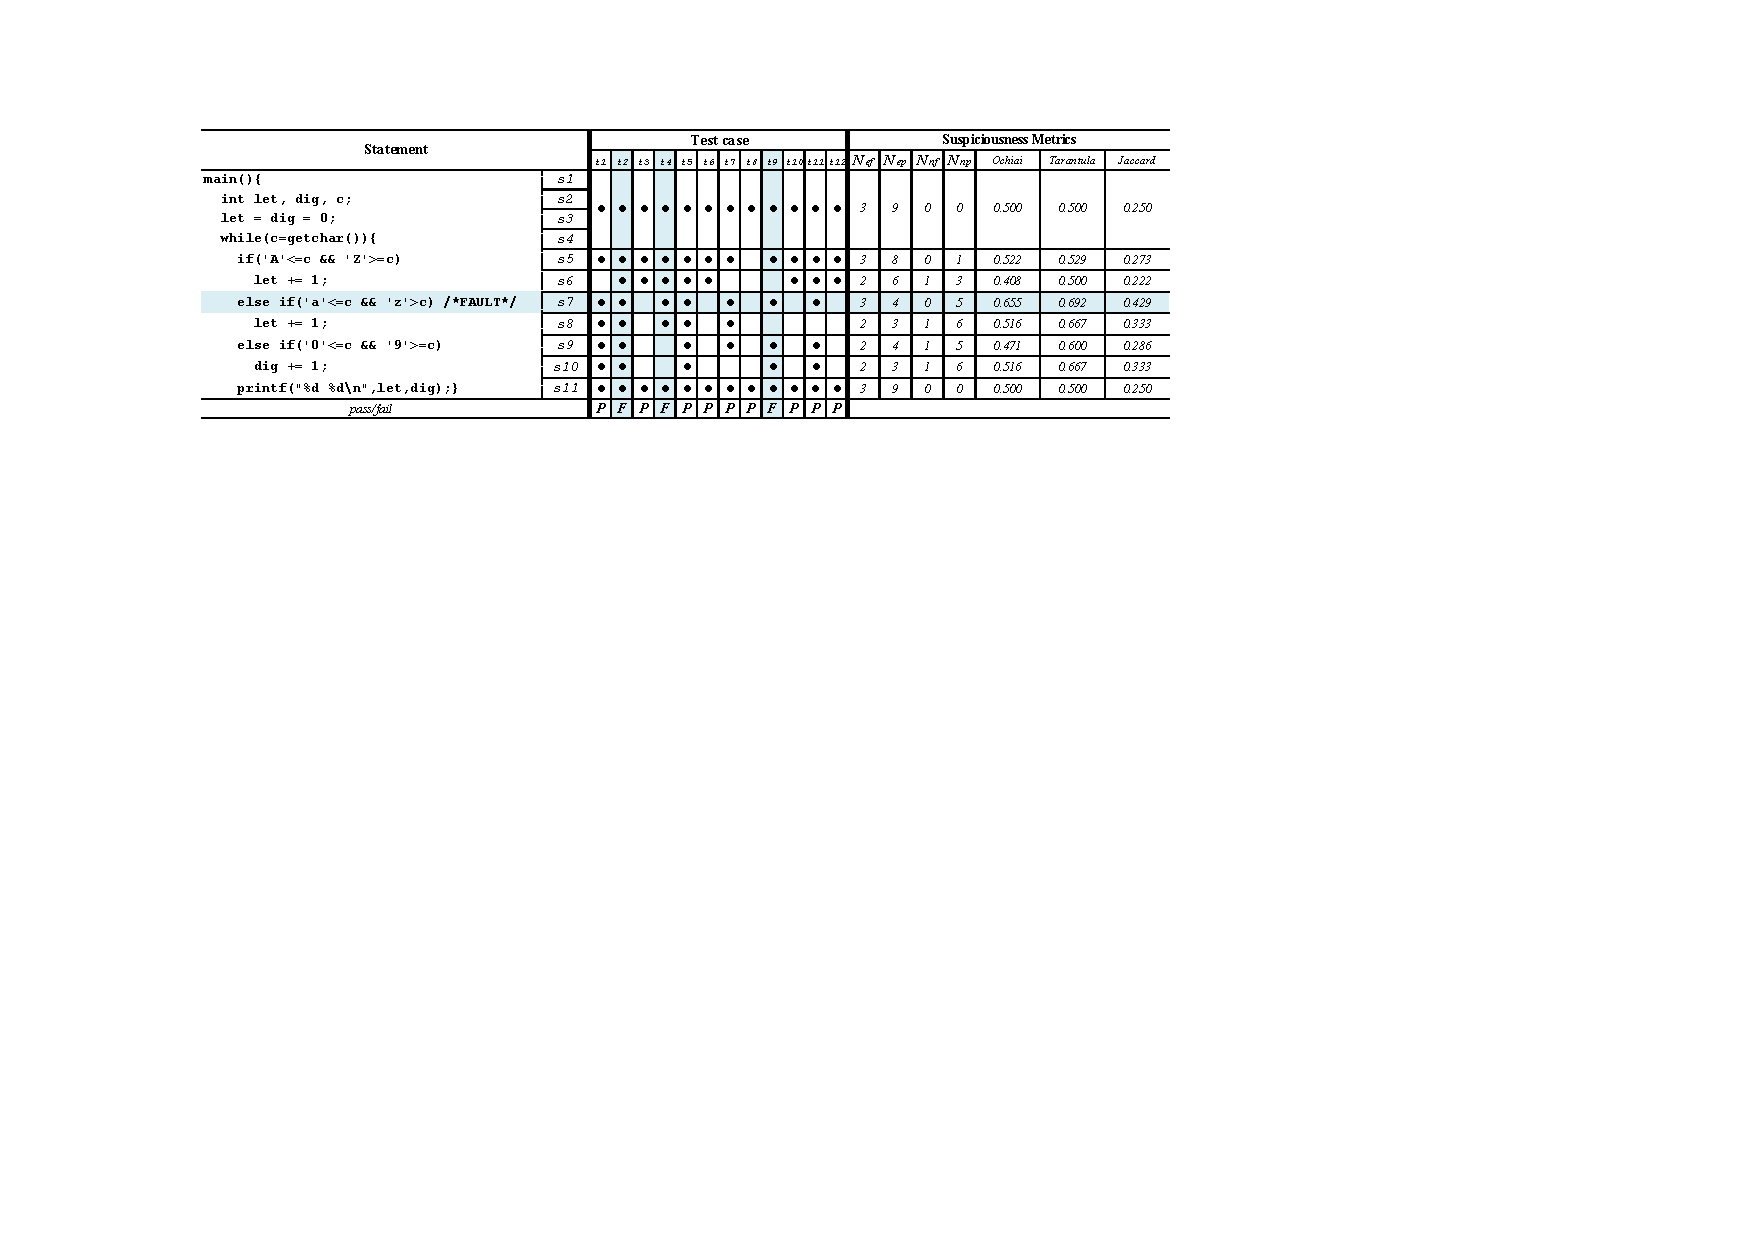
\includegraphics[width=13cm]{motivating_example.pdf}
  }
  \subfigure[Evolution of Suspiciousness Scores with Test Cases Selected by our approach]{
    \label{tab:dms_evo}
\hspace*{-20pt}
    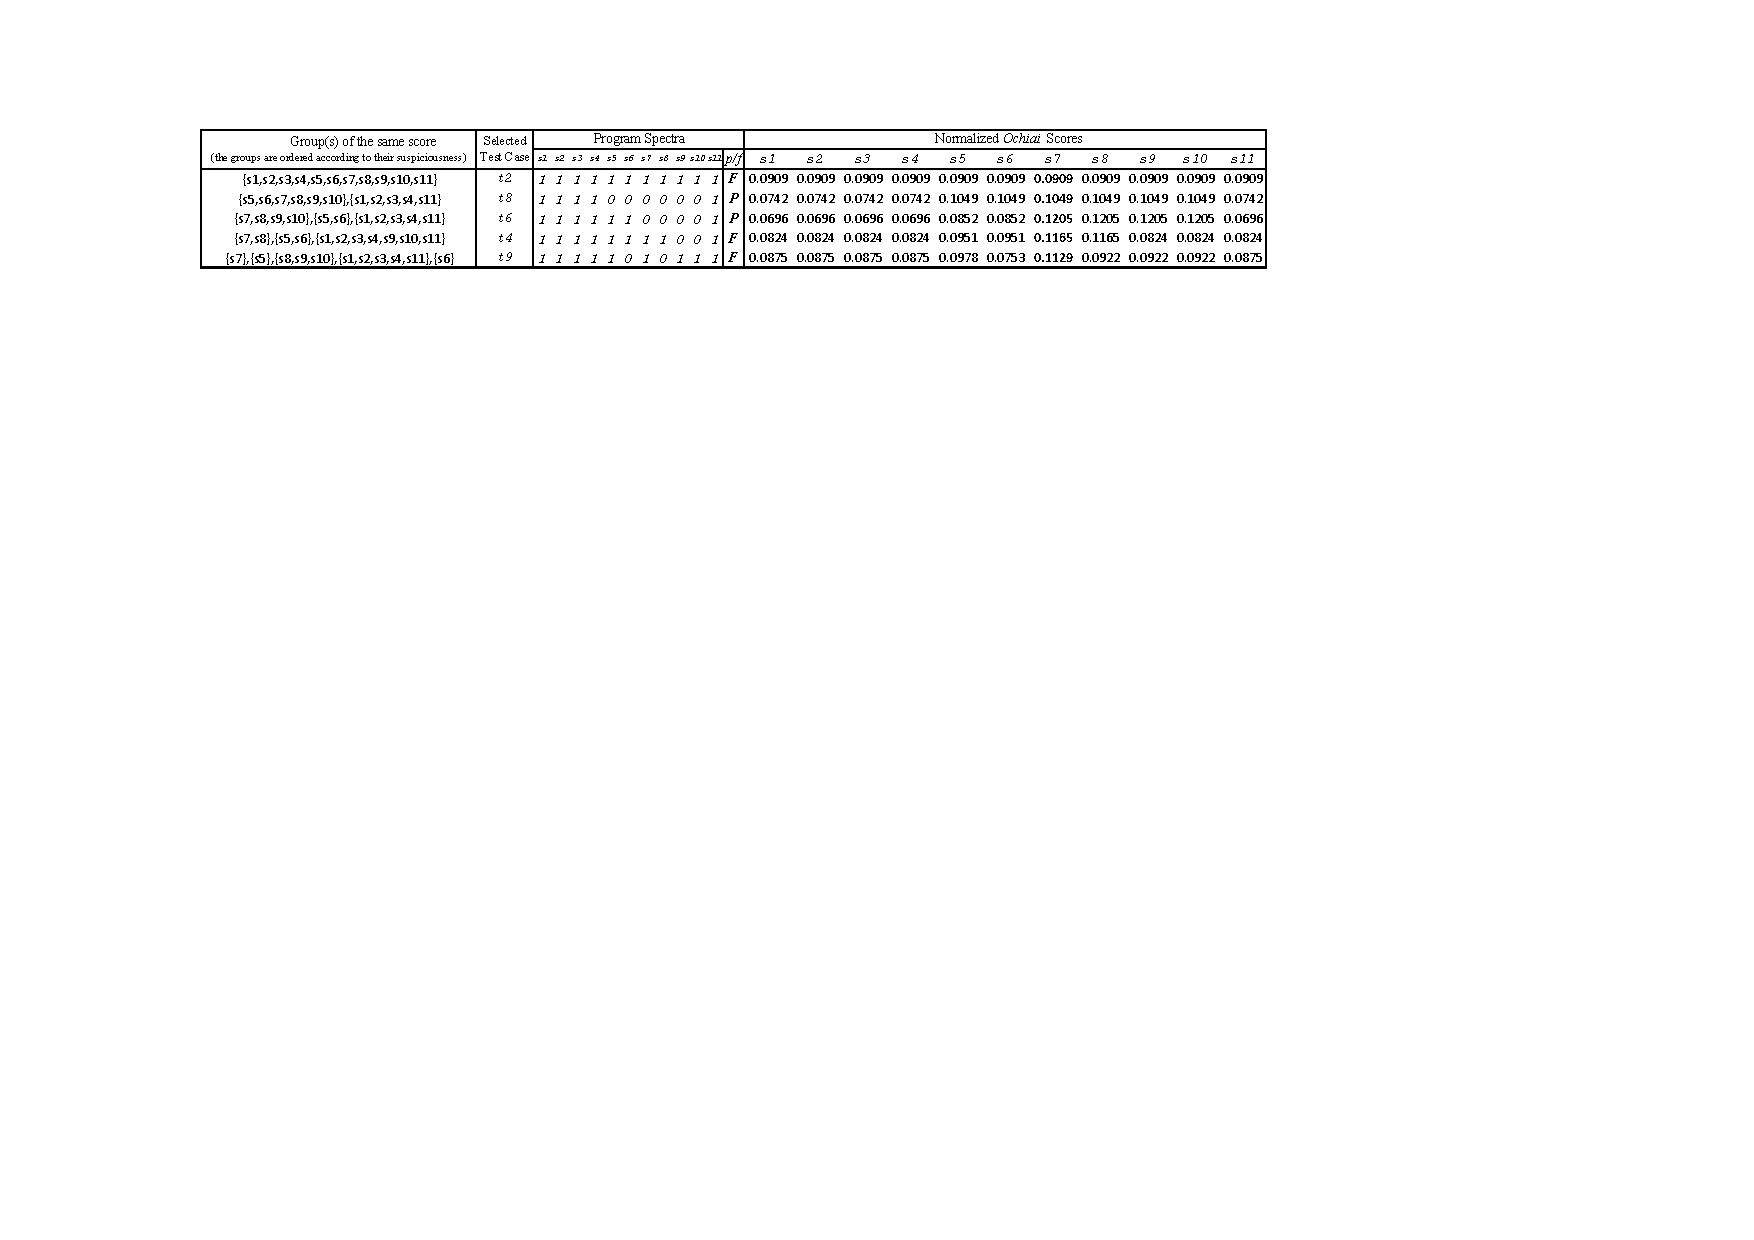
\includegraphics[width=13cm]{our_table.pdf}
  }
  %\vspace*{-16pt}
  \caption{Running Example}
  \label{fig:motiv-example}
\end{figure}

%Essentially, {\sc Dms} aims to use as few test cases as possible to quickly exhibit different characteristics among different program elements and help fault localization techniques to discriminate fault elements from non-faulty ones. Then, the human labeling effort is only needed for the much reduced test cases.
Figure~\ref{motiv_example} and~\ref{tab:dms_evo} illustrate how our concept helps reduce the number of test cases while maintaining the effectiveness of fault localization techniques.

There are 11 statements $s_{1},...,s_{11}$ in the program in Figure~\ref{motiv_example} (adapted from previous papers \citep{Gonzalez-SanchezPAGG11,JiangCT11}), where $s_{7}$ is faulty. Suppose the program has 12 test cases $t_{1},...,t_{12}$. A dot for a statement under a test case means the corresponding statement is executed (or hit) in the corresponding test case. The collection of such dots (or represented as sequences of \texttt{\textit{1}} and \texttt{\textit{0}} as shown in Figure~\ref{tab:dms_evo}) are called {\em program spectra}. With the spectra for all of the test cases and their pass/fail information, fault localization techniques may calculate various suspiciousness scores for each of the statements and rank them differently. In this case, three well-known techniques, {\em Ochiai}~\citep{Abreu:2009.jss}, {\em Tarantula}~\citep{JH05}, and {\em Jaccard}~\citep{Abreu:2009.jss} all rank $s_{7}$ as the most suspicious statement (the last three columns in the highlighted row for $s_{7}$ in Figure~\ref{motiv_example}). However, the fault localization techniques can in fact achieve the same effectiveness (i.e., ranking $s_{7}$ as the top suspicious one) with much fewer test cases when our concept is applied.

Use {\em Ochiai} as an example. First, we select an initial small number of test cases ($t_{2}$ in the example). After a programmer labels the execution result of $t_{2}$, {\em Ochiai} can already assign a suspiciousness score to each statement, although the ranks are not accurate (as in the last 11 columns of the row for $t_{2}$ in Figure~\ref{tab:dms_evo}). Then, our approach calculates the potential rank changes that may be caused if a new test case is used by {\em Ochiai}, and selects the next test case with the maximal change potential ($t_{8}$ in our case) for manual labeling. With a label for $t_{8}$, {\em Ochiai} updates the suspiciousness scores for the statements (as in the last 11 columns of the row for $t_{8}$). Repeating such a process three more times, test cases $t_{6}$, $t_{4}$ and $t_{9}$ are added, and {\em Ochiai} can already rank $s_{7}$ as the most suspicious statement. Thus, our approach helps {\em Ochiai} to effectively locate the fault in this case with only five test cases, instead of 12. Section~\ref{sec.problem} and~\ref{sec.approach} present more details about our approach.

\subsection{Contributions}

We have evaluated our approach on five real {\em C} programs and seven Siemens test programs from the Software-artifact Infrastructure Repository (SIR~\citep{doESE05}).
In total, we analyze 411 faults. 254 of them are in single-fault versions from these 12 programs, while the other 157 faults are in 173 versions of 8 of these programs.
The results demonstrate that our approach
%significantly 
outperforms existing test case selection methods for fault localization.

%\vspace{-5pt}
\begin{enumerate}
	\setlength{\parskip}{0pt}%
    \setlength{\itemsep}{3pt}%
	\item Given a target fault localization accuracy, our approach can significantly reduce the number of test cases needed to achieve it. In particular, we compare with several state-of-the-art test case prioritization strategies, including coverage-based (e.g., {\sc Stmt-Total}~\citep{RUCH01,SEAGMGR01}, {\sc Art}~\citep{JiangZCT09}), fault-exposing potential based~\citep{RUCH01}, and {\em diagnostic prioritization}~\citep{Alberto2011,Gonzalez-SanchezPAGG11,JiangCT11}, and our approach achieves, on average, test case reduction rates from
10\% to 96\% for single-fault programs, and 6\% to 67\% for multi-fault programs.
	\item Given a maximum number of test cases that a programmer can manually label (i.e., given a fixed number of test cases to be used for fault localization or a testing budget), {\sc Dms} can improve the accuracy of fault localization and thus helps reduce the amount of code programmers need to investigate to locate faults and reduce testing and debugging cost. In comparison with other test case selection techniques, we show, with Wilcoxon signed-rank test~\citep{WF1943} at 95\% confidence level, that the cost saving achieved by {\sc Dms} is statistically significant on real-life programs.
\end{enumerate}

\subsection{Paper Outline}

% Paper structure
The rest of this paper is organized as follows: Section~\ref{sec.prelim} describes fault localization and test case prioritization techniques that we use in our study. Section~\ref{sec.problem} formally introduces the problem we address. Section~\ref{sec.approach} presents our approach in detail. Section~\ref{sec.experiment} presents our empirical evaluation. Section~\ref{sec.related} describes more related works.
Finally, Section~\ref{sec.conclusion} concludes with future work.
